\documentclass[a4paper,12pt]{report}

\newcommand{\nameInitial}{\textcolor{black}{D.H. von Eschwege}}
\newcommand{\nameFull}{\textcolor{black}{Daniel von Eschwege}}
\newcommand{\stNumber}{\textcolor{black}{21785155}}
\newcommand{\myDate}{\textcolor{black}{\today}}
\newcommand{\signature}{frontmatter/fig/Signature}


% Page layout
\usepackage[left=2.2cm,right=2.2cm,top=2.2cm,bottom=2.2cm]{geometry}

% Figures
\usepackage[margin=\the\parindent,small,bf,sf]{caption}
\usepackage{graphicx}
\usepackage[section]{placeins}
\usepackage{pdfpages}
\setlength{\abovecaptionskip}{7.5pt}  % spacing above and below captions
\newcommand*{\WaterMark}[2][0.2\paperwidth]{\AddToShipoutPicture*{\AtTextCenter{\parbox[c]{0pt}{\makebox[0pt][c]{\includegraphics[width=#1]{#2}}}}}}
\usepackage{subcaption}
\setlength{\belowcaptionskip}{-5pt}
 \usepackage{wrapfig}

% Font and text-
\usepackage[afrikaans,english]{babel}
\usepackage{microtype}
\usepackage{setspace}
\usepackage{lmodern}
\newcommand{\myemph}[1]{{\sffamily\bfseries#1}}
\sloppy
\onehalfspacing
\usepackage{siunitx}
\usepackage{lipsum}


% Headings
\usepackage[raggedright,sf,bf]{titlesec}
\titlelabel{\thetitle.\ }
\titleformat{\chapter}[display]{\huge\bfseries\sffamily}{\chaptertitlename\ \thechapter}{15pt}{\raggedright}
% \titleformat{\chapter}[display]{\centering\huge\bfseries\sffamily}{\chaptertitlename\ \thechapter:}{15pt}{}
\titlespacing*{\chapter}{0pt}{0pt}{10pt}  % remove spacing before chapter headings

% Table of contents
\makeatletter
\let\originall@chapter\l@chapter
\def\l@chapter#1#2{\originall@chapter{{\sffamily #1}}{#2}}
\makeatother
\let \savenumberline \numberline
\def \numberline#1{\savenumberline{#1.}}

% Mathematics
\usepackage[cmex10]{amsmath}
\usepackage{amssymb}
\usepackage{cancel}
\usepackage{multicol}
\DeclareMathOperator*{\argmax}{arg\,max}
\newcommand{\T}{^\textrm{T}}
\newcommand{\tr}{\textrm{tr}}
\renewcommand{\vec}[1]{\boldsymbol{\mathbf{#1}}}
\newcommand{\defeq}{\triangleq}
\usepackage{gensymb}

% Tables
\usepackage{booktabs}
\usepackage{tabularx}
\usepackage{multirow}
\newcommand{\mytable}{
    \centering
    \small
    \renewcommand{\arraystretch}{1.2}
    }
\renewcommand{\tabularxcolumn}[1]{m{#1}}
\newcolumntype{C}{>{\centering\arraybackslash}X}
\newcolumntype{L}{>{\raggedright\arraybackslash}X}

% Header and footer
\usepackage{fancyhdr}
\pagestyle{fancy}
\fancyhf{}
\renewcommand{\sectionmark}[1]{\markright{\normalsize \thesection.\ #1}}
\fancyhead[C]{\nouppercase{\textit{\rightmark}}}
\fancyhead[RO]{\thepage}
% \fancyhead[LE]{\thepage}  % double-sided printing
\fancyfoot{}
\setlength\headheight{14.5pt}
\renewcommand{\headrulewidth}{0pt}
\fancypagestyle{plain}{\fancyhead{}
                       \renewcommand{\headrulewidth}{0pt}
                       \fancyfoot[C]{\thepage}}

% Pseudo-code
\usepackage{algorithm}  % should go before \usepackage{hyperref}

% Table of contents and hyperlinks
\usepackage{hyperref}
\hypersetup{colorlinks=true,linktoc=all,citecolor=black,linkcolor=black}
\usepackage[nottoc]{tocbibind}

% Pseudo-code
\usepackage{algpseudocode}  % should go after \usepackage{hyperref}
\renewcommand{\thealgorithm}{\arabic{chapter}.\arabic{algorithm}} 
\captionsetup[algorithm]{labelfont={bf,sf},font=small,labelsep=colon}

% Bibliography
\usepackage{cite}  % automatically reorder inline citations
\bibliographystyle{IEEEtran}

% Fix titlesec issue
\usepackage{etoolbox}
\makeatletter
\patchcmd{\ttlh@hang}{\parindent\z@}{\parindent\z@\leavevmode}{}{}
\patchcmd{\ttlh@hang}{\noindent}{}{}{}
\makeatother

\setlength{\parindent}{0pt}

\begin{document}

% Front matter
\graphicspath{{frontmatter/fig/}}
\pagenumbering{Alph}

\begin{titlepage}
\begin{center}


\includegraphics[width=10cm]{USlogo-top}

\vfill

{\sffamily \bfseries \huge E344 Assignment 3 \par}

\vfill

{\large {\Large \nameFull} \\ \stNumber \par}

\vfill

\vfill

{Report submitted in partial fulfilment of the requirements of the module \\
Design (E) 344 for the degree Baccalaureus in Engineering in the Department of
Electrical and Electronic Engineering at Stellenbosch University. \par}

\vfill

%{\large {Supervisor}: Dr L. Skywalker} %\\
% Department of Electrical and Electronic Engineering \par}

\vfill

{\Large \myDate}
\end{center}
\end{titlepage}

\pagenumbering{roman}
%\chapter*{Declaration}
\newpage
\pagestyle{plain}
\addcontentsline{toc}{chapter}{Declaration}
\makeatletter\@mkboth{}{Declaration}\makeatother

\centerline{
\includegraphics[width=8cm]{USlogo-top}}
\vspace*{-10pt}

\section*{\centering Plagiaatverklaring / \textit{Plagiarism Declaration}}

\vspace*{5pt}

\begin{enumerate}
    \item Plagiaat is die oorneem en gebruik van die idees, materiaal en ander intellektuele eiendom van ander persone asof dit jou eie werk is.\\
    \textit{Plagiarism is the use of ideas, material and other intellectual property of another's work
        and to present is as my own.}
    
    \item Ek erken dat die pleeg van plagiaat 'n strafbare oortreding is aangesien dit 'n vorm van diefstal is.\\
    \textit{I agree that plagiarism is a punishable offence because it constitutes theft.}
    
    \item Ek verstaan ook dat direkte vertalings plagiaat is. \\
    \textit{I also understand that direct translations are plagiarism.}
    
    \item Dienooreenkomstig is alle aanhalings en bydraes vanuit enige bron (ingesluit die internet) volledig verwys (erken). Ek erken dat die woordelikse aanhaal van teks sonder aanhalingstekens (selfs al word die bron volledig erken) plagiaat is. \\
    \textit{Accordingly all quotations and contributions from any source whatsoever (including the internet) have been cited fully. I understand that the reproduction of text without quotation marks (even when the source is cited) is plagiarism}
    
    \item Ek verklaar dat die werk in hierdie skryfstuk vervat, behalwe waar anders aangedui, my eie oorspronklike werk is en dat ek dit nie vantevore in die geheel of gedeeltelik ingehandig het vir bepunting in hierdie module/werkstuk of 'n ander module/werkstuk~nie. \\
    \textit{I declare that the work contained in this assignment, except where otherwise stated, is my original work and that I have not previously (in its entirety or in part) submitted it for grading in this module/assignment or another module/assignment.}
\end{enumerate}

\vfill

\noindent \begin{tabularx}{1.0\linewidth}{|L|L|}
    \hline
    \hspace{2cm} \large{\stNumber}& \vspace{4mm}\hspace{2cm} \includegraphics[height=1.5cm]{\signature}\\

    \vspace{0mm}{Studentenommer / \textit{Student number}} & \vspace{0mm} {Handtekening / \textit{Signature}} \\
    \hline
    \vspace{1mm}  \hspace{2cm} \large{\nameInitial} & \vspace{1mm} \hspace{2cm} \large{\myDate }\\
    \vspace{1mm} {Voorletters en van / \textit{Initials and surname}} & \vspace{1mm} {Datum / \textit{Date}} \\
    \hline
\end{tabularx}

\vspace{15pt}




\tableofcontents
\listoffigures
\listoftables
\chapter*{Nomenclature\markboth{}{Nomenclature }}
\addcontentsline{toc}{chapter}{Nomenclature}


\textcolor{red}{update these}
% \vspace*{-3mm}
\subsubsection*{Variables and functions}

\begingroup
\renewcommand{\arraystretch}{1.2}
\renewcommand{\tabularxcolumn}[1]{p{#1}}
\begin{tabularx}{\textwidth}{@{}p{2.5cm}L}
    $p(x)$ & Probability density function with respect to variable $x$.\\
    $P(A)$ & Probability of event $A$ occurring.\\
    $\varepsilon$ & The Bayes error. \\
    $\varepsilon_u$ & The Bhattacharyya bound. \\
    $B$ & The Bhattacharyya distance. \\
    $s$ & An HMM state.  A subscript is used to refer to a particular state, e.g.\ $s_i$ refers to the $i^{\text{th}}$ state of an HMM. \\
    $\mathbf{S}$ & A set of HMM states. \\
    $\mathbf{F}$ & A set of frames. \\
    $\mathbf{o}_f$ & Observation (feature) vector associated with frame $f$. \\
    $\gamma_s(\mathbf{o}_f)$ & A posteriori probability of the observation vector $\mathbf{o}_f$ being generated by HMM state $s$. \\
    $\mu$ & Statistical mean vector. \\
    $\Sigma$ & Statistical covariance matrix. \\
    $L(\mathbf{S})$ & Log likelihood of the set of HMM states $\mathbf{S}$ generating the training set observation vectors assigned to the states in that set. \\
    $\mathcal{N}(\mathbf{x} | \mu, \Sigma)$ & Multivariate Gaussian PDF with mean $\mu$ and covariance matrix $\Sigma$.\\
    $a_{ij}$ & The probability of a transition from HMM state $s_i$ to state $s_j$. \\
    $N$ & Total number of frames or number of tokens, depending on the context. \\
    $D$ & Number of deletion errors. \\
    $I$ & Number of insertion errors. \\
    $S$ & Number of substitution errors. \\
\end{tabularx}
\endgroup


\newpage
\subsubsection*{Acronyms and abbreviations}
\textcolor{red}{update this}\\
\begingroup
\renewcommand{\arraystretch}{1.2}
\begin{tabular}{@{}p{2.5cm} l}
    AE      & Afrikaans English \\
    AID     & accent identification \\
    ASR     & automatic speech recognition \\
    AST     & African Speech Technology \\
    CE      & Cape Flats English \\
    DCD     & dialect-context-dependent \\
    DNN		& deep neural network \\
    G2P     & grapheme-to-phoneme \\
    GMM     & Gaussian mixture model \\
    HMM     & hidden Markov model \\
    HTK     & Hidden Markov Model Toolkit \\
    IE      & Indian South African English \\
    IPA     & International Phonetic Alphabet \\
    LM      & language model \\
    LMS     & language model scaling factor \\
    MFCC    & Mel-frequency cepstral coefficient \\
    MLLR    & maximum likelihood linear regression \\
    OOV     & out-of-vocabulary \\
    PD      & pronunciation dictionary \\
    PDF     & probability density function \\
    SAE     & South African English \\
    SAMPA   & Speech Assessment Methods Phonetic Alphabet \\
\end{tabular}
\endgroup

\newpage
\pagenumbering{arabic}

% Contents

\chapter{System design}
\section{System overview} \label{sec:system}

\begin{figure}[h]
    \centering
    \vspace{-0.7cm}
    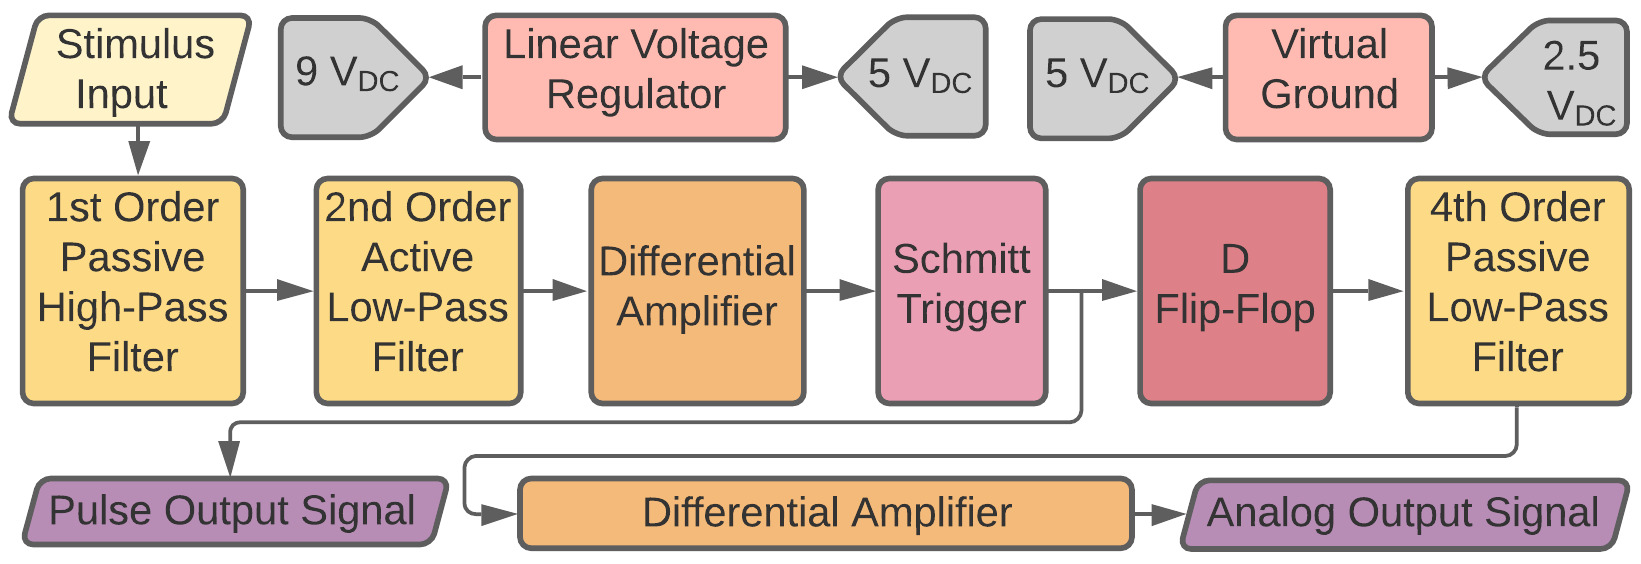
\includegraphics[width = 1\textwidth]{Figures/overview}
    \caption{System Diagram}
    \label{fig:overview}
\end{figure}

Creating a health monitoring system requires the design and implementation of a heart-rate sensor. This sensor obtains an input signal, from which pulses, corresponding to heart-beats are generated, as well as analogue values which represent the heart-rate. The aforementioned is achieved by means of various subcircuits, respectively responsible for voltage regulation, signal conditioning, pulse generation and conversion to analogue, which proceeds as can be seen in figure \ref{fig:overview} - explanation follows hereafter.
A voltage regulator generates 5 V which powers the circuit. See \ref{ } old report for the design. The stimulus input signal, obtained from the heart-rate sensor, is to be converted to a pulse output signal, but has an amplitude of insufficient magnitude, and is subject to high levels of noise. This necessitates signal conditioning: the input signal is fed into a first order passive high-pass filter and a second-order active low-pass filter consecutively, thereby attenuating both high- and low-frequency noise. The filters were chosen with maximal simplicity in mind, as to reduce cost and complexity, while still performing adequately. After filtering, the signal is amplified by means of a differential amplifier, resulting in a signal with a large amplitude and little noise. This allows for pulse generation by means of a Schmitt Trigger comparator, which produces an output pulse signal, where the frequency corresponds to the heart-rate. The Schmitt Trigger was preferred above alternatives as it provides a a noise margin by means of hysteresis, thereby eliminating heart-beat misdetections that otherwise arise. Further, an analogue voltage is required, where the voltage level represents the heart-rate. Filtering and peak detection using diodes was considered, but ultimately discarded, as diodes are non-linear, resulting in extremely slow simulation. Rather, the pulse output signal was converted to a pulse-width modulated signal, where the frequency of the former determined the duty cycle of the latter. This was done as PWM signals lend themselves to conversion-to-analogue by simple filtering. The PWM signal was obtained by using a D Flip-Flop in conjunction with a RC-circuit (see section \ref{•} for more detail), and was then filtered by a fourth-order passive RC filter. Passive components were selected as to reduce current usage and simulation time. The filter is of high order as to greatly minimize noise, as the settling time requirement for the analog signal was easily met.

\pagebreak


Also point the reader to your first report for more information on the temperature sensing and voltage regulation, and use a citation to it (add it to your \texttt{References.bib} file and cite it here). Remember to state what your remaining power budget is, based on Assignment 1's results. 










\chapter{System design}
\section{System overview} \label{sec:system}

\begin{figure}[h]
    \centering
    \vspace{-0.7cm}
    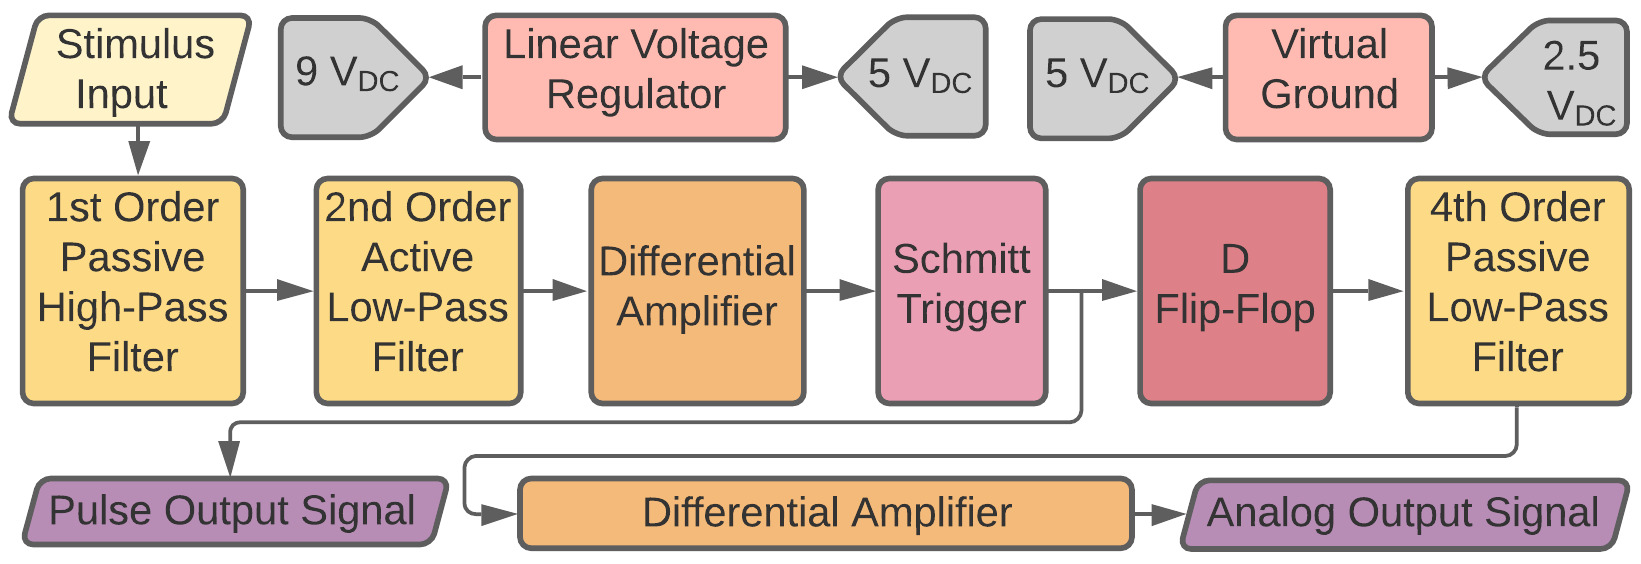
\includegraphics[width = 0.9\textwidth]{Figures/overview}
    \caption{System Diagram}
    \label{fig:overview}
\end{figure}


\chapter{Temperature sensor conditioning circuit}\label{sec:temp_sensor}

%**********************************************
\section{Intro} \label{sec:temp_intro}
%**********************************************
The signal obtained from the temperature sensor presents as DC, with a \SI{35}{\milli \volt}, \SI{50}{Hz} AC signal superimposed, which serves no purpose, but creates noise. The DC component increases linearly with respect to the temperature measured by the sensor. However, the sensor outputs a voltage of \SI{440}{\milli \volt} at 0\degree C, which increases by \SI{35}{\milli \volt} for every 1\degree C. These voltage levels are too small for a microcontroller ADC to take as input. Furthermore, as the sensor is only meant to measure human body temperature, the applicable range is only from 34\degree C to 42\degree C. The two aforementioned considerations necessitate amplification of the relevant part of the temperature sensor signal to occupy as much of a \numrange{0}{5} \si{\volt} range as possible, as this is the voltage range used by the ADC.
To this end, a temperature sensor conditioning circuit is required to transform the given input into the desired output. This conditioning circuit consists of a filter, an offset removing subcircuit, as well as an amplifier. The filter attenuates the AC signal present in the input signal in order to obtain an output signal with a minimal amount of noise. The offset removing subcircuit removes enough of the DC offset to ensure that the output signal is centered around \SI{2.5}{\volt}, which is necessary to obtain the largest possible output swing as discussed previously. Finally, the amplifier increases the magnitude of the input signal in order to be suitable as input for an ADC.

%**********************************************
\section{Design}\label{sec:temp_design}
%**********************************************
The amplifier was designed first, as its gain serves as the determining factor for the amount of noise reduction that is required from the filter. A TLC2272 op-amp was chosen as it allows for an output very close to its rails. Since the output signal has to be centered around \SI{2.5}{\volt}, a differential amplifier was decided upon, as the negative input can be used to adjust the offset present in the output. Given a zero-reference temperature sensor voltage ($V_{zero}$) of \SI{440}{\milli \volt}, with an increase ($V_{\Delta}$) of \SI{35}{\milli \volt} for every 1\degree C. Therefore, temperature sensor voltage levels are calculated as follows: $V_{temp} = V_{zero} + V_{\Delta} \times \mathrm{Temp}$ 

%Table \ref{tab:temp} shows some of the relevant voltage levels:

\begin{table}[h]
        \centering
        \footnotesize
        \caption{Temperatures and Corresponding Voltage Levels}
         \begin{tabular}{c@{\qquad}rrr}
          \toprule
          Temperature [\degree C] 	& 32    & 38	& 42\\
          Voltage [V] 			& 1.63	& 1.77	& 1.91\\
          \bottomrule
        \end{tabular}
     \label{tab:temp}
\end{table}

According to table \ref{tab:temp}, the maximum input voltage swing equals $1.91 - 1.63 = 0.28$V, and has a DC offset of \SI{1.77}{\volt}. Amplification is needed to reach an output voltage swing of \SI{5}{\volt}. Therefore:

$$A_v = \frac{V_{out}}{V_{in}} = \frac{5}{0.28} = 17.86$$

Considering the current design requirement of \SI{25}{mA} maximum, the input resistor R is selected as \SI{10}{\kilo \Omega}, which will therefore, at the highest possible voltage level (\SI{5}{\volt}), use \SI{0.5}{mA} of current.  This gives $R_{feedback} = 178.6$k$\Omega$, according to $A_v = \frac{{R}_{feedback}}{R}$ \cite{opamp}. R corresponds to $R_1$ and $R_2$, and $R_{feedback}$ to $R_{3}$ and $R_4$ in the final design diagram (figure \ref{fig:final}), which is shown here already to aid with the explanation of the design process. 

\begin{figure}[H]
    \centering
    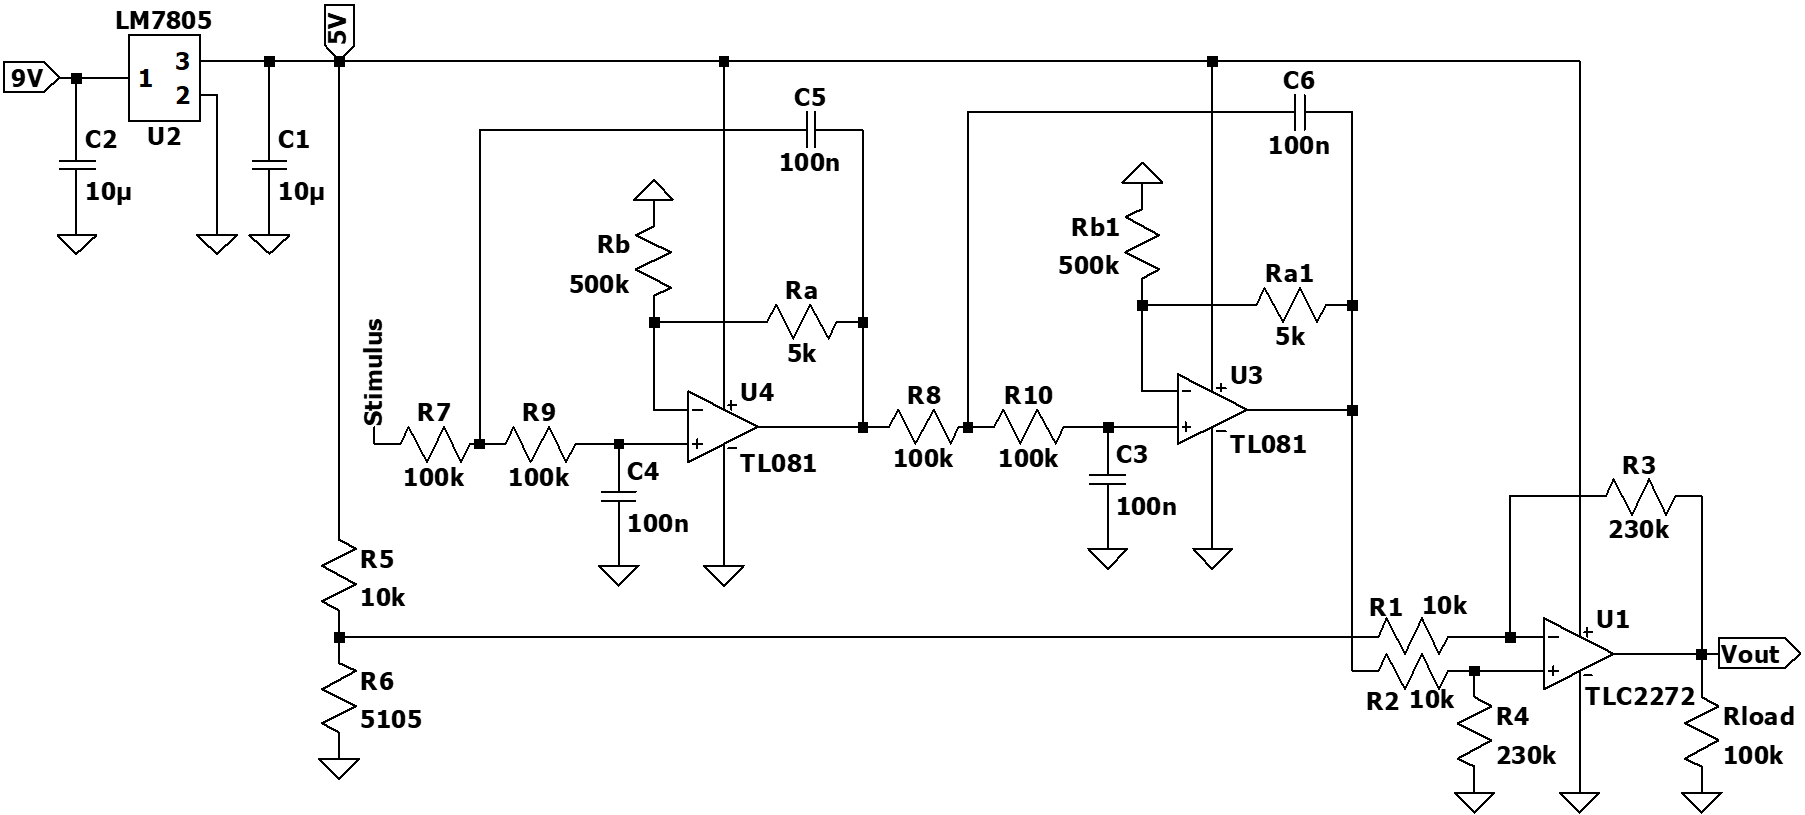
\includegraphics[width = 1\textwidth]{Figures/final.png}
    \caption{Temperature Sensor Circuit}
    \label{fig:final}
\end{figure}

Two points need to be considered: 
\begin{enumerate}
\item The DC offset of the input signal is undesired and has to be removed in order to obtain a zero-mean input signal. This can be achieved by designing another subcircuit that makes use of another op-amp, for example. This adds to the cost and complexity of the circuit.
\item The output signal has to be centered around \SI{2.5}{\volt}. This means that a DC offset has to be added in the form of a virtual ground.
\end{enumerate}

When considered in conjunction with each other, the DC offset alteration can be resolved in one step, thereby reducing cost and complexity significantly. The decision was therefore made to use a differential amplifier, with the input signal connected to the positive input, after which the voltage required at the negative input can be calculated in such a way as to simultaneously subtract the offset and add the virtual ground in one step, thereby producing an output DC offset of \SI{2.5}{\volt} (the lecturer mentions that this is an acceptable approach in Lecture Video 2).  This approach also simplifies the design procedure, as it becomes unnecessary to calculate the virtual ground separately. The differential amplifier, however, has to be non-inverting. The calculation thus reduces to a simple differential amplifier gain formula \cite{opamp}: 

$$V_{out}=\frac{{R}_{feedback}}{{R}}\left({V}_{in+}-{V}_{in-}\right) \;\;\; \rightarrow \;\;\; 2.5=\frac{178600}{10000}\left(1.77-{V}_{in-}\right)$$

With $V_{out}$ as \SI{2.5}{\volt}, $V_{in+}$ as \SI{1.77}{\volt} and the resistor values as calculated previously, ${V}_{in-} = 1.63 \; \mathrm{V}$. The voltage at ${V}_{in-}$ can be set by means of a voltage divider circuit, which takes \SI{5}{\volt} as input and is calculated as follows (resistor names in formulae are selected to conform with Figure \ref{fig:final}):

$${V}_{in-} = 5 (\frac{R_{6}}{R_{6}\times R_{5}})$$

Selecting $R_5$ as \SI{10}{\kilo \Omega} gives $R_6 =$ \SI{4.84}{\kilo \Omega}.\\

The filter has to be designed next. Possible design choices included an active/passive first order low-pass filter, a simple RC filter, or a second order low-pass filter. Simulation of the aforementioned filters has shown the following: the RC filter is very simple, but does not meet the design requirements w.r.t. noise. The passive low-pass filter is relatively simple, but does not meet the settling time requirement. The active low-pass filter meets both the noise and settling time requirements, but requires the TLC2272 op-amp to do so. Since a single TLC2272 op-amp is more expensive than multiple TL081 op-amps, the decision was made to rather use cascaded second order low-pass filters, which  make use of the TL081. This is somewhat more complex, but lowers the cost, as the final circuit now only uses three op-amps, two of which are the cheaper TL081 models. The cascaded setup also produces an output signal with extremely low noise.  A filter gain of close to unity is desired; for $R_A = $ \SI{500}{\kilo\Omega}, a value of \SI{5}{\kilo\Omega} is suitable for $R_A$, according to the formula from \cite{filter}:

$${A_v}=1+\frac{{R}_A}{R_B}$$

The settling time requirement of \SI{100}{ms} means that a cutoff frequency of more than \SI{10}{Hz} is needed, while the attenuation of noise requires a cutoff frequency below \SI{50}{Hz}. In order to minimize noise, the cutoff frequency was selected at \SI{15}{Hz} - the bandwidth thus also is \SI{15}{Hz} (only positive frequencies considered). Choosing R ($\mathrm{R_7 \; and \; R_9}$ in the diagram) as \SI{100}{\kilo\Omega} gives C ($\mathrm{C_4 \; and \; C_5}$) as \SI{106.1}{nF}, according to

$$f_c=\frac{1}{2 \pi RC}$$

The given cutoff frequency implies a rise time of \SI{19.1}{ms} according to $t_{r} \approx \frac{1.8}{w_{n}} = \frac{1.8}{2 \pi (15)}$\cite{cs}. This meets the requirement of \SI{100}{ms}. After design completion, this filter is then duplicated and connected back-to-back in order to form cascaded second-order low-pass filters, as seen in figure \ref{fig:final}.\\

Under most circumstances, it is a good design practice to include a unity gain op-amp at the input of the op-amp responsible for the correct offset, as it acts as a voltage buffer, thereby clamping the voltage against fluctuations caused by the differential amplifier's other input. This design practice was considered, but ultimately decided against, as tests with and without the buffer provided outputs of equal quality (similar to the output shown in section \ref{sec:temp_results}). The reason a buffer is not needed is due to the signal conditioning circuit already having a very high input resistance, following from the choice of resistors. The only notable differences resulting from the inclusion of a buffer were an increase in current drawn, as well as an increase in cost for the circuit components, as another op-amp is required. Therefore, in order to keep the current consumption below \SI{15}{mA}, as well as to use reduce cost by only using three op-amps, the voltage buffer was omitted in the final design. 


%**********************************************
\section{Results} \label{sec:temp_results}
%**********************************************
The designed circuit produces a signal centered at \SI{2.5}{\volt} with an output swing of \SI{4.86}{\volt} (figure \ref{fig:vout}), exceeding the required \SI{3.5}{\volt}. The absolute maximum amount of noise measured is \SI{25.6}{\milli\volt}, and the settling time is \SI{67}{ms}, thereby meeting the requirements of \SI{50}{\milli\volt} and \SI{100}{ms} respectively. Total current draw is \SI{12.83}{mA}, well below the required \SI{15}{mA}. The cutoff frequency, obtained via AC analysis simulation, is \SI{10.48}{Hz} (figure \ref{fig:ac}). Measurements and graphs of settling time, cutoff frequency and current drawn can be seen in Appendix C. It is thus clear that all requirements, as well as all bonus requirements, have been met with a good margin to spare, all the while using only three op-amps, two of which are the cheaper TL081 models. The output signal (light blue) is shown in figure \ref{fig:vout}.

\begin{figure}[h]
    \centering
    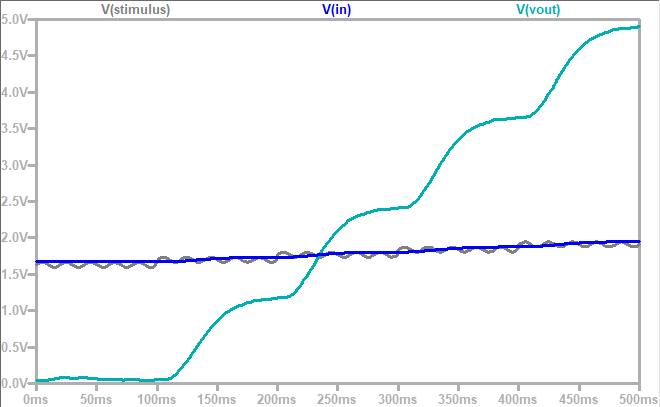
\includegraphics[width = 1\textwidth]{Figures/vout.png}
    \caption{Temperature Sensor Conditioning Circuit Output}
    \label{fig:vout}
\end{figure}

%**********************************************
\section{Summary}\label{sec:temp_summary}
%**********************************************
Concluding, the circuit performs very well, and successfully amplifies the temperature sensor output to a level that is readable by the microcontroller ADC, all the while attenuating almost all noise present in the input. The design is somewhat complex, but also cheaper, as it uses less of the TLC2272 op-amps.



\chapter{Heart rate sensor}\label{ch:heartRate}
%**********************************************

%**********************************************
\section{Introduction} \label{sec:heartIntro}
%**********************************************
Circuits pertaining to signal conditioning, pulse signal and analogue output generation will be discussed. Conditioning is done via filtering and amplification, thereafter thresholding and pulse-width modulation is used to generate outputs. Active filters provide high input and low output impedance, and a large Q-factor \cite{actpas}. A differential amplifier is suitable for amplification, as the gain is referenced against a customizable voltage \cite{opamp}. A Schmitt Trigger is well-suited for pulse generation, as it provides a noise margin \cite{schmitt}. PWM signals can be converted to analogue using filtering \cite{PWM}.

%**********************************************
\section{Design} \label{sec:heartDesign}
%**********************************************
\begin{figure}[h]
    \centering
    \vspace{-1cm}
    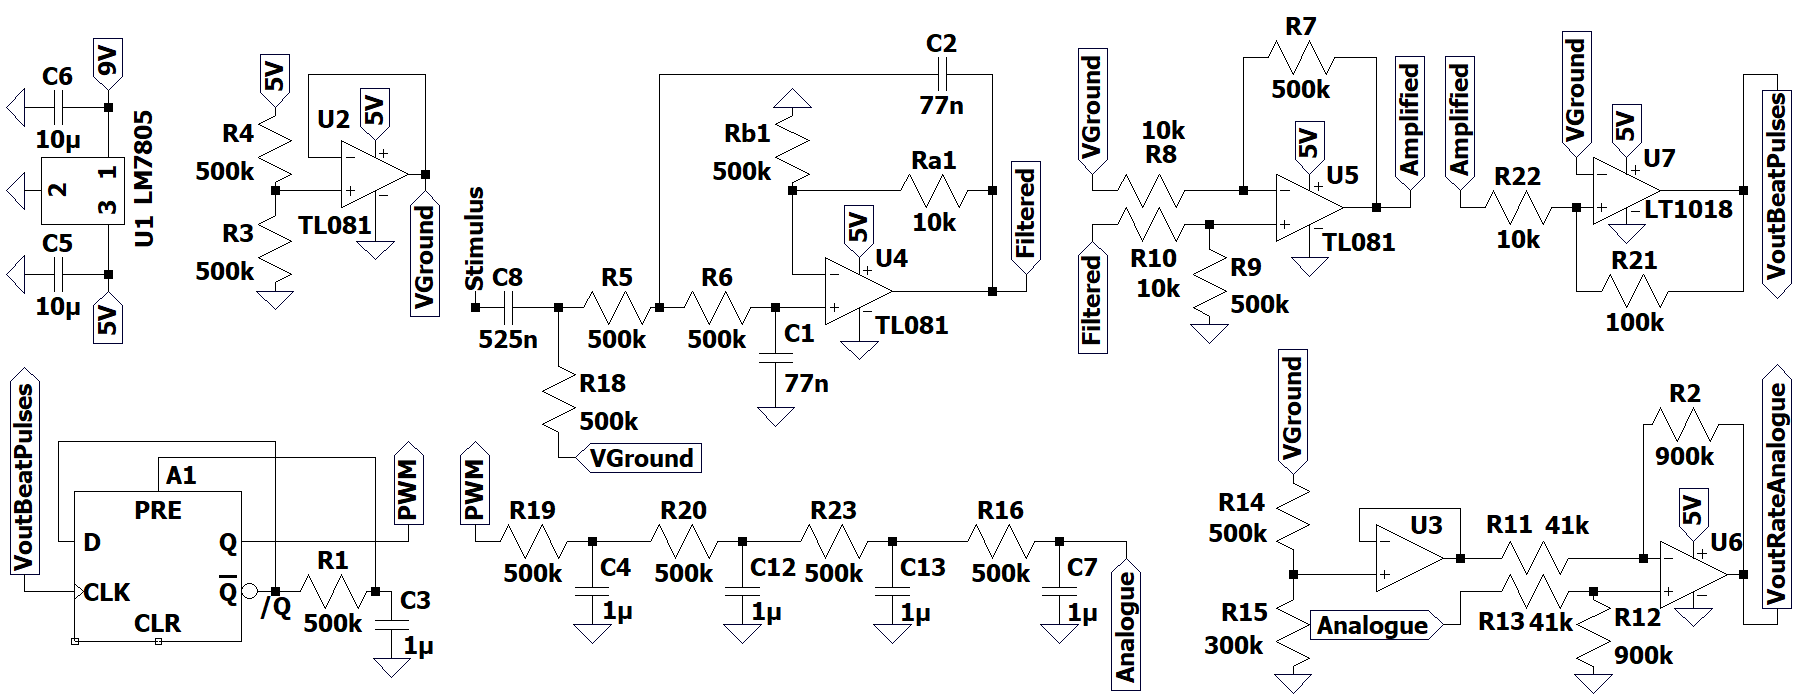
\includegraphics[width = 1\textwidth]{Figures/circuit}
    \caption{Complete Circuit}
    \label{fig:circuit}
\end{figure}

The complete circuit is shown upfront in figure \ref{fig:circuit} to aid explanation. The largest resistor in sub-circuits is always chosen to be \SI{500}{k\Omega} as to reduce current usage. The TLC2272 op-amp has $V_{CM}$ of \numrange{-0.3}{4} \si{V}, $V_{ID} = \pm 16 \; V$, $V_{in_{max}} = V_{DD+}$ and $V_{in_{min}} = V_{DD-} - 0.3$ \cite{tlc2272}. The TL081 has $V_{CM}$ of \numrange{1}{4} \si{V}, $V_{ID} = \pm 30 \;V$, $V_{in_{max}} = 3.5 \;V$ and $V_{in_{min}} = 1.5 \;V$ \cite{tl081}. This information is given here as to avoid repetition - refer here when op-amp characteristics are discussed. The design process now follows.
The FFT of the stimulus input in figure \ref{fig:fft} shows information residing between \numrange{0.8}{2.5} \si{Hz}, corresponding to 50 and 150 BPM respectively. The other peaks represent noise at \SI{0.25}{Hz}, as well as at twice and three times the message signal, and higher. Noise distorts square wave output, necessitating filtering. 
\begin{wrapfigure}{r}{0.5\textwidth}
%	\vspace{-0.45cm}
    \centering
    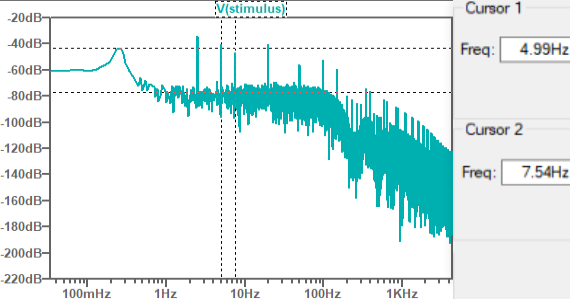
\includegraphics[width = 0.44\textwidth]{./Figures/fft}
%	\vspace*{-1mm}
    \caption{Fast fourier transform of stimulus}
    \label{fig:fft}
\end{wrapfigure}
A first order passive high-pass filter, $f_c =$ \SI{0.606}{Hz}, attenuates the low frequency noise at \SI{0.25}{Hz}. R18 = \SI{500}{k\Omega}, thus C8 = \SI{525}{nF} according to $f_{c} = \frac{1}{2\pi R C}$. A virtual ground centres the signal around \SI{2.5}{V}, ensuring that the LPF input falls within the common-mode range of the TL081, which is used as it inexpensive \cite{octo}. A second order active low-pass filter, $f_c =$ \SI{4.1}{Hz}, filters out high frequency noise. R5 = R6 = \SI{500}{k\Omega}, C1 = C2 = \SI{77}{nF} - see aforementioned formula. Cutoff frequencies were selected to remove noise maximally while minimally affecting heart-rate data. The signal should reside slightly above \SI{2.5}{V} to facilitate amplification (to be discussed) and to ensure common-mode input range compliance in the next stage. Thus, Rb1 = \SI{500}{k\Omega} and Ra1 = \SI{10}{k\Omega} since $A_v=1+\frac{R_{A}}{R_{B}}$ 
\cite{filter}. A filter output with DC offset slightly above \SI{2.5}{V} allows for the use of a differential amplifier with the existing virtual ground connected to the negative input, removing the need for additional circuitry otherwise required. The signal is amplified according to $\mathrm{V}_{\mathrm{OUT}}=\frac{\mathrm{R}_{a}}{\mathrm{R}_{b}}\left(\mathrm{V}_{2}-\mathrm{V}_{1}\right)$ \cite{opamp}, where R\textsubscript{a} corresponds to R7 and R9 and R\textsubscript{b} to R8 and R10. The gain of 50 was selected to again provide a DC offset of \SI{2.5}{V}, as it facilitates implementation of the comparator (to be discussed). Since the amplified signal has an amplitude of only \SI{1.66}{V}, the inexpensive TL081 was chosen despite having a smaller output range. Next, the signal is fed into a Schmitt Trigger - the LT1018 comparator allows for output very close to 0 and 5V and has a high gain. \SI{5}{V} is produced if the input exceeds the upper trip point (UTP) and \SI{0}{V} if the input falls below the lower trip point (LTP) \cite{schmitt}. The hysteresis width ($w_h =$ UTP - LTP) serves as a noise margin around the reference voltage, $V_{REF}$ \cite{schmitt}. The DC offset of \SI{2.5}{V} of the amplified signal requires $V_{REF}$ = \SI{2.5}{V}, once again allowing for the use of the existing virtual ground. Pulse duration is designed for the highest frequency, as it will then also meet the requirement for lower frequencies. Since 150 BPM corresponds to a period of \SI{0.4}{s}, $w_h$ should be selected to ensure an output pulse width of at least \SI{150}{ms}; \SI{200}{ms} selected to account for noise. The amplified signal approximates a sinusoid:

\noindent\begin{minipage}{.5\linewidth}
\vspace{-0.35cm}
\begin{equation}
    y_1 = 1.66\sin(2\pi(2.5)t_1) + 2.5
    \label{eq:sin1}
\end{equation}
\end{minipage}%
\begin{minipage}{.5\linewidth}
\vspace{-0.35cm}
\begin{equation}
    y_2 = 1.66\sin(2\pi(2.5)t_2) + 2.5
    \label{eq:sin2}
\end{equation}
\end{minipage}

Subtracting \ref{eq:sin2} from \ref{eq:sin1} yields $y_1 - y_2 = w_h =$ \SI{0.52}{V} for $t_1 =$\SI{0.01}{s} and $t_2 =$ \SI{.
21}{s}, resulting in a theoretical pulse width ranging from \numrange{0.2}{0.625} \si{ms}, which is sufficient. $w_h$ also is an order of magnitude larger than the highest input signal noise levels, increasing design fidelity.  Now, UTP = \SI{2.75}{V}, LTP = \SI{2.25}{V}, UTP = $V_{REF} + \beta Vcc$ and LTP = $V_{REF} - \beta Vcc$, thus $\beta$ = 0.05 \cite{schmitt}. Further, $\beta=\frac{\mathrm{R}_{22}}{\mathrm{R}_{22}+\mathrm{R}_{21}}$. Thus R21 = \SI{190}{k\Omega} and R22 = \SI{10}{k\Omega}. (R21 was adjusted to \SI{100}{k\Omega} to account for loading effects). A one-shot was considered to extend the pulses, but was omitted as it was superfluous. The pulse output frequency thus represents the heart-rate.\\

Obtaining an output suitable for a microcontroller presents itself as a problem of converting frequency to analogue. The decision was made to obtain a PWM signal from the FM pulse signal, as PWM signals readily lend themselves to conversion-to-analogue using a simple low-pass RC filter. Pulse-width modulation was achieved by means of a D flip-flop. The essence of the design is to firstly keep the output high continually, but to then drive the output low for a fixed time, once per period. Since the period of the clock signal varies against BPM, driving low for a fixed amount of time results in a different ratio of the pulse being low at different frequencies, producing a varying duty cycle. Specifically, the previously generated pulse signal is used as a clock signal for the D flip-flop, and the not-Q output is fed back into the data line. This would normally drive the output high for all time $t$; thus a RC circuit is added of which the capacitor is charged by the not-Q output, and connected to the SET-line of the flip-flop. Once the capacitor charges to \SI{2.5}{V}, Q is pulled high and not-Q low until the next rising edge of the clock input inverts Q and not-Q. The result is a slightly delayed PWM signal, with a large duty cycle at high frequencies, and vice-versa. The result is a consistent PWM output, as long as the capacitor charge time is selected to be shorter than the narrowest pulse of the clock signal. See section \ref{sec:heartResults}, figure \ref{subfig:pwm} for output. Calculations follow. R1 = \SI{500}{k\Omega} gives $C = 1\mu$, according to the capacitor charge/discharge exponential equations - the extended solution (via Matlab scripting) is given in Appendix \ref{app:} for the sake of brevity. Having obtained a PWM signal, a fourth order passive low-pass filter produces analogue values in the range of \numrange{0.95}{1.2} \si{V}. A cutoff frequency of \SI{0.5}{Hz} ensures maximal attenuation of noise while maintaining a 5\% settling time of 10 seconds. Therefore R = \SI{500}{k\Omega} and C = \SI{1}{\mu}. Finally, the analogue output is amplified by means of a TLC2272 differential amplifier with a negative input at \SI{0.938}{V}. A gain of 20 produces a sufficient output range. Resistor values were increased as to minimize loading effects - thus R2 = R12 = \SI{900}{k\Omega} and R11 = R13 = \SI{45}{k\Omega} according to $\mathrm{V}_{\mathrm{OUT}}=\frac{\mathrm{R}_{a}}{\mathrm{R}_{b}}\left(\mathrm{V}_{2}-\mathrm{V}_{1}\right)$ \cite{opamp}. Loading effects still had a slight effect, and required adapting R11 and R13 to \SI{41}{k\Omega}. An analogue transducer is thus designed. For microcontroller integration, a log-linear scale can linearise the analogue output, and the calibration constant is calculated. The slope is $\frac{0.8-2.5}{4.7-0.5} = -0.404$. Thus, for 150 BPM, $f = 2.5 = -0.404V + C = -0.404(0.5) + C \;\;\; \rightarrow \;\;\; C = 2.702$.\\
Total current is calculated using \SI{1.4}{mA} per TL081 \cite{tl081}, \SI{2.2}{mA} per TLC2272 \cite{tlc2272} and \SI{110}{\mu A} per LT1018 \cite{lt1018}. Non-trivial resistors are all approximated using \SI{5}{V} over, as to err on the side of caution: $4(1.4m) + (2.2m) + (110n) + 16\left(\frac{5}{500k}\right) + 3\left(\frac{5}{10k}\right) +
 2\left(\frac{5}{41k}\right) + \left(\frac{5}{100k}\right) =$ \SI{9.75}{mA}. Voltage regulator current is considered in E344 Assignment 1 \cite{prev}. $100m - 9.75m - 11.39m$ leaves \SI{78.86}{mA} for Assignment 3.

%**********************************************
\section{Results} \label{sec:heartResults}
%**********************************************

\begin{wrapfigure}{r}{0.38\textwidth}
\centering
\vspace{-.8cm}
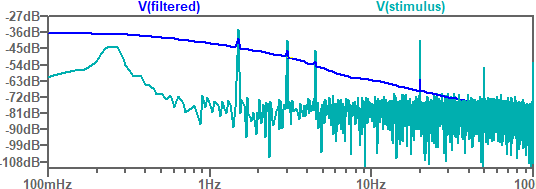
\includegraphics[width=0.38\textwidth]{./Figures/filtout}
%\vspace*{1mm}
\caption{Filter input and output}
\label{fig:filtout}
\end{wrapfigure}

The frequency response of the high- and low-pass filters gives $-3dB$ at \SI{0.61}{Hz} and $-6dB$ at \SI{4.3}{Hz} respectively - see figures \ref{subfig:hpf} and \ref{subfig:lpf1}. This reflects design calculations near perfectly. Comparison of filter input and output in figure \ref{fig:filtout} shows a drastic noise reduction.
\pagebreak

\begin{figure}[h]
 \footnotesize
   \centering
   \begin{subfigure}[]{0.48\textwidth}
        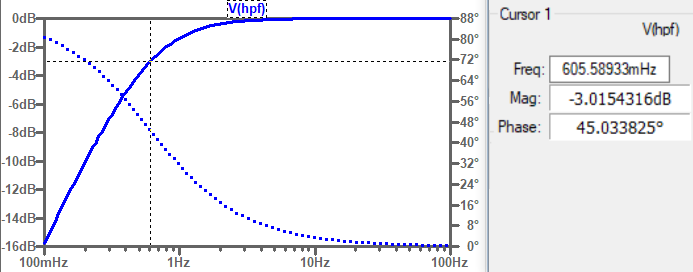
\includegraphics[width=\linewidth]{./Figures/hpf}
	  \caption{High-pass filter} \label{subfig:hpf}	
   \end{subfigure}
   \begin{subfigure}[]{0.48\textwidth}
  	 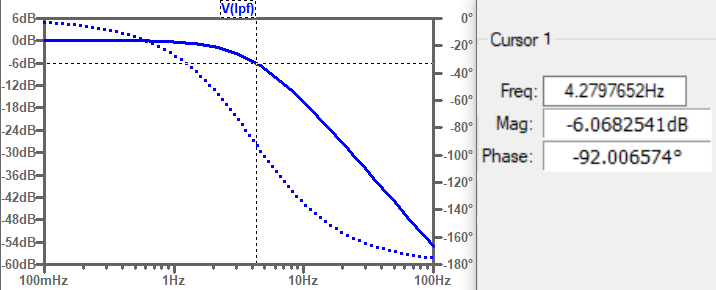
\includegraphics[width=\linewidth]{./Figures/lpf1}
	  \caption{Second-order low-pass filter} \label{subfig:lpf1}	
   \end{subfigure}
   \caption {Frequency response of filters}
   \label{fig:freqreq}
 \end{figure}

The filtered signal is passed through a differential amplifier; the input is shown in blue and the output in red in figure \ref{subfig:amplified}. The filtered signal has a \SI{50}{mV} amplitude (peak-to-peak), and the output \SI{1.747}{V}. Therefore $A_v \approx 35$, which, although smaller than calculated, is to be expected due to non-linear behaviour for high amplification factors. Input and output of a LT1018 comparator, used for thresholding, is shown in figure \ref{subfig:pulses}.  See UTP = \SI{2.75}{V} and LTP = {2.25}{V} in figure \ref{subfig:pulses}, giving a hysteresis width of \SI{0.5}{V}, exactly as calculated.

\begin{figure}[h]
 \footnotesize
   \centering
   \begin{subfigure}[]{0.49\textwidth}
        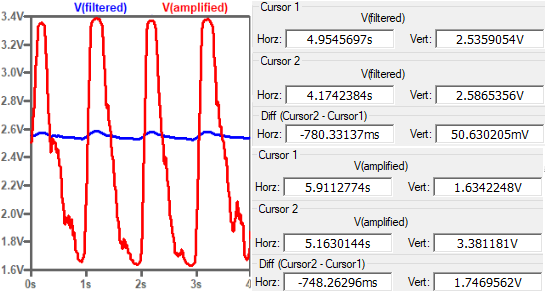
\includegraphics[width=\linewidth]{./Figures/amplified}
	  \caption{Amplification of filtered signal} \label{subfig:amplified}	
   \end{subfigure}
   \begin{subfigure}[]{0.49\textwidth}
  	 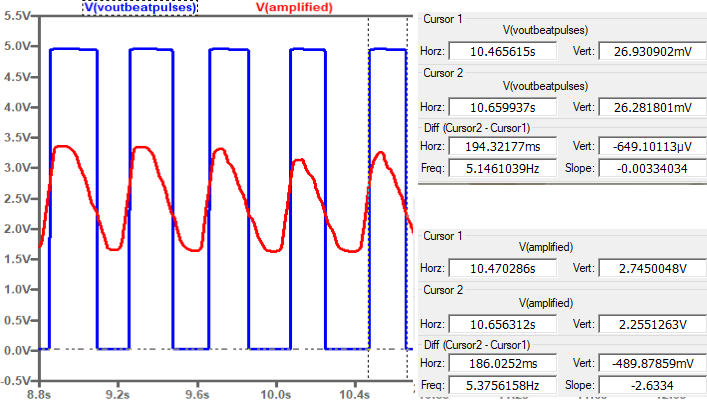
\includegraphics[width=\linewidth]{./Figures/pulses}
	  \caption{Thresholding} \label{subfig:pulses}	
   \end{subfigure}
   \caption{Signal Conditioning}
 \end{figure}
 
The output ranges from \numrange{0.026}{4.95}\si{V}, with a pulse duration in range \numrange{189}{584} \si{ms} in figures \ref{subfig:pulses2} and \ref{subfig:pulses1}, meeting the \SI{150}{ms} requirement. The design remains consistent for specification deviations of $\pm 10\%$ amplitude and a DC offset variation of $\pm$ \SI{0.2}{V}, as the high-pass filter removes the DC component and the filter has a cutoff frequency low enough to greatly attenuate noise.

\begin{figure}[h]
 \footnotesize
   \centering
   \begin{subfigure}[]{0.49\textwidth} 	 
  	 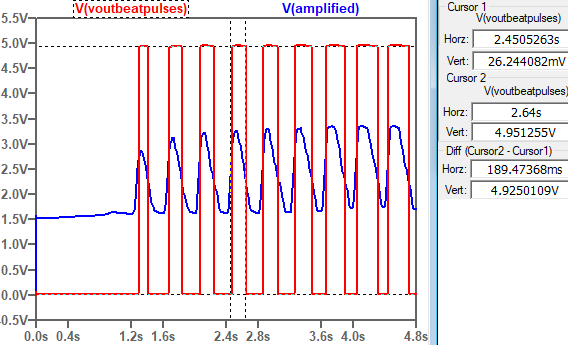
\includegraphics[width=\linewidth]{./Figures/pulses2}
	  \caption{150 BPM} 
	  \label{subfig:pulses2}	
   \end{subfigure}
   \begin{subfigure}[]{0.49\textwidth}
        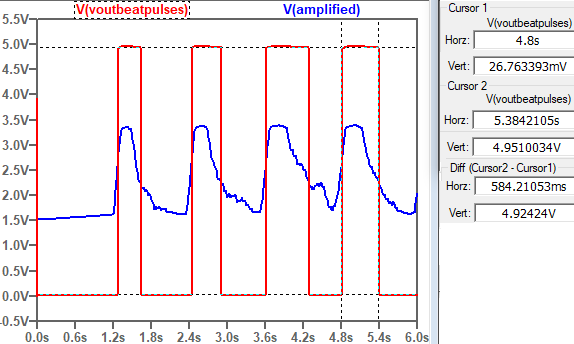
\includegraphics[width=\linewidth]{./Figures/pulses1}
	  \caption{50 BPM} 
	  \label{subfig:pulses1}	
   \end{subfigure}
   \caption{Full input versus output range}
 \end{figure}

\pagebreak
For the analogue transducer, a PWM signal is obtained. Section \ref{sec:heartDesign} explains the interrelation, where \texttt{voutbeatpulses, pwm} and \texttt{rc} in figure \ref{subfig:pwm} correspond to the clock signal, Q, and the charging capacitor voltage respectively. The 5\% settling time is \SI{9.45}{s}. The duty cycle is 73\% at 60 BPM and decreases to 56\% at 150 BPM. Finally, amplification and filtering of the PWM signal produces analogue output, range \SI{4.2}{V} (\ref{subfig:analog}).

\begin{figure}[h]
 \footnotesize
   \centering
   \begin{subfigure}[]{0.57\textwidth}
        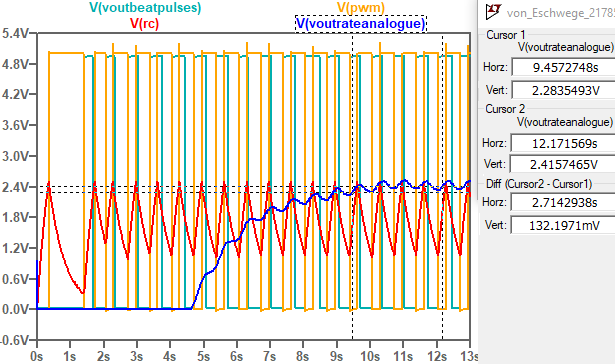
\includegraphics[width=\linewidth]{./Figures/pwm}
	  \caption{PWM and settling time} 
	  \label{subfig:pwm}	
   \end{subfigure}
   \begin{subfigure}[]{0.41\textwidth}
  	 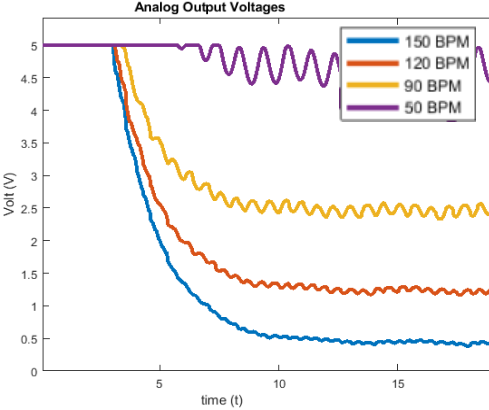
\includegraphics[width=\linewidth]{./Figures/analog}
	  \caption{Analogue voltage output} 
	  \label{subfig:analog}	
   \end{subfigure}
 \end{figure}

\begin{wrapfigure}{r}{0.55\textwidth}
\centering
\vspace{-0.3cm}
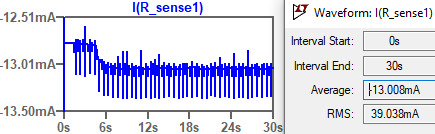
\includegraphics[width=0.55\textwidth]{./Figures/current}
\caption{Total current usage}
\label{fig:current}
\end{wrapfigure}
In figure \ref{fig:current}, total current draw is measured through R\textsubscript{sense}, averaging \SI{13.0}{mA}, meeting the bonus requirement of \SI{15}{mA}. When combined with Assignment 1, the combined current of \SI{25.8}{mA} still is far less than the maximum current rating of \SI{100}{mA} for the voltage regulator \cite{prev}. 

%**********************************************
\section{Summary}\label{sec:temp_summary}
%**********************************************
Concluding, it has been shown that the design performs as expected, meeting the all requirements. Output pulse width is broader than required, analogue output is generated with discrete, non-overlapping values exceeding the required range, while settling to a final value according to specification.  Current draw remains sub-\SI{15}{mA}. Upon implementation of the microcontroller, be cognizant of the fact that analogue output values scale in a slightly non-linear fashion. This is not a problem, as it can be easily accounted for in software. By design, the system is limited to the 50 to 150 BPM range, but could be expanded using the existing design as a proof-of-concept. 


\chapter{Calibration and digitisation}\label{ch:ADC}

\section{Temperature sensor} \label{sec:ADCTemp}

	\subsection{Analytical Design} \label{sec:ADCTempAna}

Equation \ref{eq:temp} for the sensor voltage and \ref{eq:amp} for the amplifier, where the addition of a virtual ground and offset correction are combined by $V_{offset}$.

\begin{equation}
\vspace{-0.4cm}
\label{eq:temp}
V_{sense} = V_{0} + \alpha(T) \;\;\; \rightarrow \;\;\; T = \frac{1}{\alpha}(V_{sense} - V_{0})
\end{equation}

\begin{equation}
%\vspace{-0.4cm}
\label{eq:amp}
V_{out}=A_{v}\left({V}_{sensor}-{V}_{offset}\right) \;\;\; \rightarrow \;\;\; {V}_{sensor} = \frac{V_{out}}{A_{v}} + V_{offset}
\end{equation}

Combining \ref{eq:temp} and \ref{eq:amp} gives

\begin{equation}
\label{eq:comb}
T = \frac{V_{out}}{\alpha A_{v}} + \frac{V_{offset} - V_{0}}{\alpha} = 1.6(V_{out}) + 34
\end{equation}

for $V_{0} =$ \SI{440}{mV}, $\alpha =$ \SI{35}{mV}, $V_{offset} =$ \SI{1.63}{V}, $A_{v} = 17.86$. For an ADC:

\begin{equation}
\label{eq:adc}
\mathrm{ADC} = (2^{10}-1)\frac{V_{in}}{V_{ref}} \;\;\; \rightarrow \;\;\; V_{in} = \frac{\mathrm{ADC}(V_{ref})}{2^{10}-1}
\end{equation}

\ref{eq:adc} into \ref{eq:comb}, with $V_{out}$ as ADC input, converts the sampled ADC value to temperature output: 

\begin{equation}
\vspace{-0.4cm}
\label{eq:adctemp}
T = (1.6)\frac{\mathrm{ADC}(V_{ref})}{2^{10}-1} + 34
\end{equation}



	\subsection{Empirical Design} \label{sec:ADCTempEmp}
\begin{wrapfigure}{r}{0.5\textwidth}
\centering
\vspace{-0.6cm}
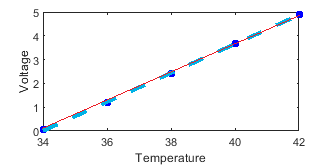
\includegraphics[width=0.5\textwidth]{./Figures/linreg}
\caption{Voltage against temperature}
\label{fig:linreg}
\end{wrapfigure}
Simulation yields the data points in figure \ref{fig:linreg}. Linear regression results the empirical equation \ref{eq:linreg}, graphed in light blue, which is implemented in software as to provide a digital temperature reading - see pseudocode below. Equation \ref{eq:adctemp} corresponds closely to the analytical equation \ref{eq:comb}, graphed in red. Python implementation yields a 1\degree C temperature reading accuracy for the full input range. 
 
\begin{equation}
\label{eq:linreg}
T = 1.644985924\left(V_{out_{avg}}\right) + 33.92887739
\end{equation}

Pseudocode:
\begin{algorithm}
V\textunderscore avg = V\textunderscore out / length(V\textunderscore out)\\
T = 1.644985924*V\textunderscore avg + 33.92887739
\end{algorithm}





\vspace{-0.7cm}
\section{Heart rate sensor}
\label{sec:ADCHeart}


	\subsection{Analytical Design} 					\label{sec:ADCTempAna}
The heart-rate signal consists of square wave pulses of which the periods correspond to the heart-rate. 



	\subsection{Empirical Design} 					\label{sec:ADCTempEmp}

Include flow diagram of code or pseudocode as a list.
No need to include the 10-bit ADC in this section. 

\chapter{System and conclusion}

\section{System}
Considering the system as a whole, it should be easy to integrate it with the rest of the health monitoring system as the design is modular. This can be done by feeding the output of the temperature sensor into the system designed in this report, and then connecting the output of the system to the microcontroller ADC. 

Concluding, it has been shown that the combination of the voltage regulator and the temperature sensing circuitry works very well to achieve the desired result. Since the cascaded filters ensure extremely low noise levels, the ADC should be capable of distinguishing the measured temperature to a very high degree of accuracy. The system uses more of the less costly components, and is very power efficient, all the while meeting all of the bonus requirements. It is thus safe to say that the objective of the design has been met successfully.

\section{System}
The design of the heart-rate sensor goes to show that a noisy input signal could effectively be converted to a square wave output as well as an analogue output, enabling reliable interfacing of real-world measurements with digital systems. The heart-rate sensing circuit can now be integrated with the remainder of the health monitoring system by connecting the analogue output to the microcontroller input, to which the temperature sensor will also be connected - see E344 Assignment 1 \cite{prev}. The modular design of different parts of the health-monitoring system simplifies both design and debugging. Due to the second order low-pass filter, the heart-rate sensor is remarkably robust with respect to variations in noise, attenuating noise levels to below 6\% of the signal amplitude before creating a pulse output. The design also performs well on a variety of the normalised input data sets. Calibration for microcontroller integration is done according to $f = -0.404V + 2.702$ (section \ref{sec:heartDesign}, and the quantisation error is $f_{err} = \frac{2.5 - 0.8}{2^{10}} / (2.5 - 0.8) \times 100 = 0.1\%$. Noise is filtered to the extent that it has a negligible effect on the digitalized reading.
The system utilizes less costly components where possible, is very power efficient, and adheres to all of the bonus requirements. The design objective has been met successfully.

\section{Lessons learnt}
1. LTSpice is a blessing, but can be an absolute nightmare with simulations. I've created a rough metric; it goes to show that 30\% of my time was spent on circuit design, 10\% on report writing, and 60\% on debugging LTSpice simulation problems. I entered E-Design with the belief that simulation would greatly accelerate the pace of the subject, as soldering was eliminated, but I stand firm in my belief that I could have built a practical circuit much faster, as 'timestep too small' does not apply in the beauty of real-world continuity. However, maybe I just stand firm in this belief because I have not dealt with the problems arising from burnt-out components, messy soldering, melted PCB tracks and exploding diodes.

2. I believe to have greatly improved with regards to modularising and debugging not only circuits, but systems in general. Treating everything as a small problem to be solved furthered my conceptual understanding of component interaction.

3. I shouldn't have gone surfing for the entirety of the first week of the term. I said this in Assignment 1 as well, and lost marks for it, but it is still applicable, so I'll say it again.

4. If I could have it all over again, I wouldn't have texted my circuit; she did not reply.


% Bibliography
\bibliography{References}

% End matter
\appendix
\chapter{Social contract}
\makeatletter\@mkboth{}{Appendix}\makeatother
\label{appen:social_contract}
\textcolor{red}{Sign and inlcude.}
%     \begin{figure}[!htb]
%     \centering
%     	\fbox{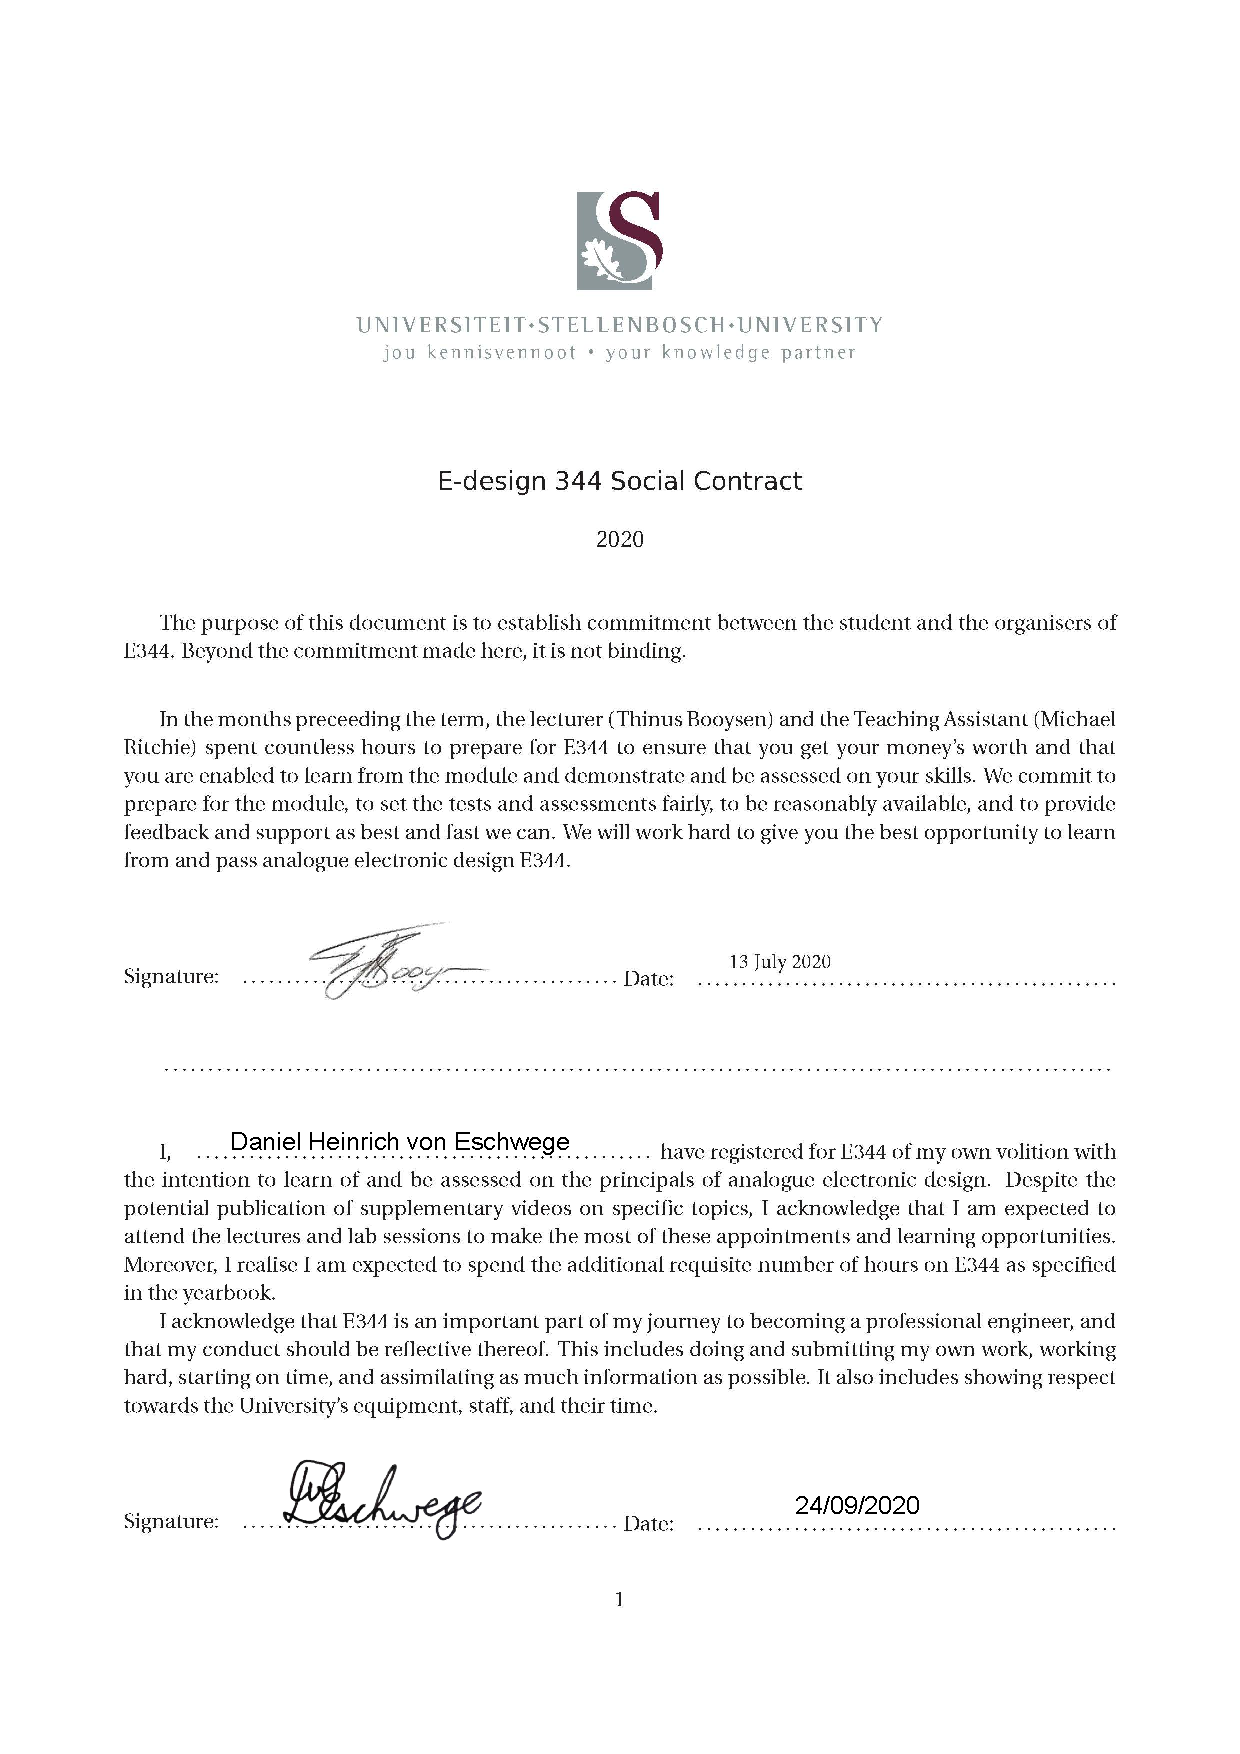
\includegraphics[width=0.78\linewidth]{./Figures/SocialContract_signed.pdf}}
%       \label{fig:social_contract}
%	\end{figure}
\chapter{GitHub Activity Heatmap}
\makeatletter\@mkboth{}{Appendix}\makeatother
\label{appen:github_heatmap}
\textcolor{red}{Take a screenshot of your github version control activity heatmap and insert here. }

     \begin{figure}[!htb]
     \centering
     	\fbox{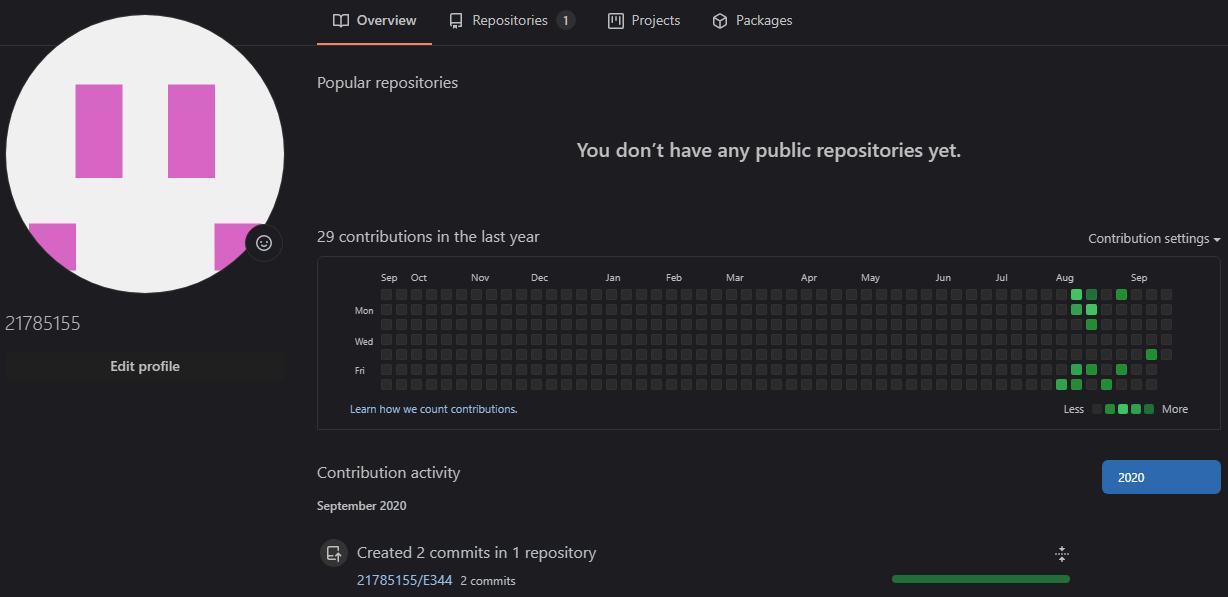
\includegraphics[width=1\linewidth]{./Figures/GitHub.png}}
	\label{fig:github}
	\end{figure}
     \chapter{Stuff you want to include}
R1 = \SI{500}{k\Omega}. $\tau = RC$. The capacitor charge oscillates between $V_L$ and $V_H$. $V_H =$ \SI{2.5}{V}. $V_L$ is reached for the first time at $t_{L_1}$ and $V_H$ at $t_{H_1}$. $V_L$ is then reached at  $t_{L_2}$. For \SI{150}{BPM} (or \SI{2.5}{Hz}), the pulse drives high for \SI{0.2}{ms}. Since the capacitor has to charge faster than \SI{0.2}{ms}, a charge time of \SI{0.16}{ms} was selected to add a 20\% margin, accounting for noise. Thus $t_{H_1} - t_{L_1} = 0.16$ and $t_{L_2} - t_{H_1} = 0.4 - 0.16 = 0.24$ for the 150 BPM signal. Finally,

$$V_L = 5\left(1-e^{\frac{t_{L_1}}{\tau}}\right)$$
$$V_H = 5\left(1-e^{\frac{-t_{H_1}}{\tau}}\right)$$
$$V_L = V_H\left(e^{\frac{t_{L_1}}{\tau}}\right)$$

giving $C = 1\mu$, when solving using the following MatLab script:\\

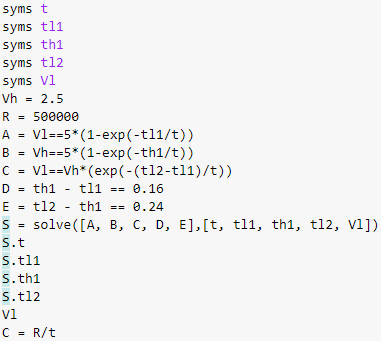
\includegraphics[width = 0.75\textwidth]{./Figures/script}
     \chapter{Stuff you want to include}

A 1\degree C step input (\SI{35}{\milli\volt}), as shown in figure \ref{subfig:ts}, was used to determine the settling time. The settling time is measured at the point where the output steps to 90\% of the final value (\SI{622}{\milli\volt}), which is \SI{560}{\milli\volt}. The settling time was thus measured as \SI{62.07}{ms}, as shown by the cursor difference in figure \ref{subfig:ts}.
\begin{figure}[h]
    \centering
    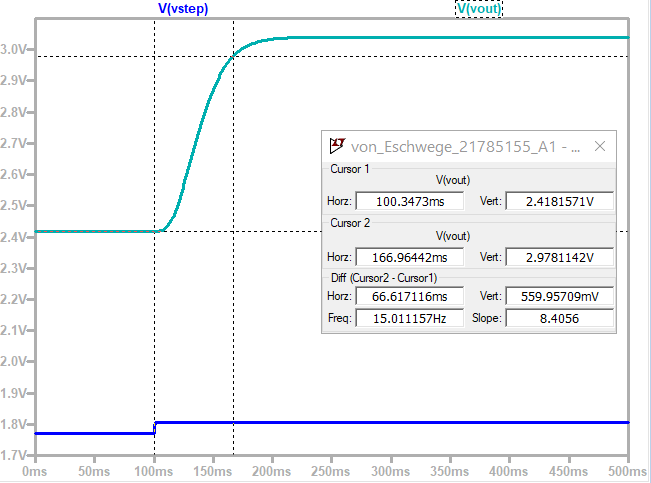
\includegraphics[width = 0.6\textwidth]{Figures/ts.png}
    \caption{Settling Time Measurement}
    \label{fig:ts}
\end{figure}

The bode plot for the low-pass filter is shown in figure \ref{fig:ac}. The -3dB point is lower than calculated, but is still well within the acceptable range. 
\begin{figure}[h]
    \centering
    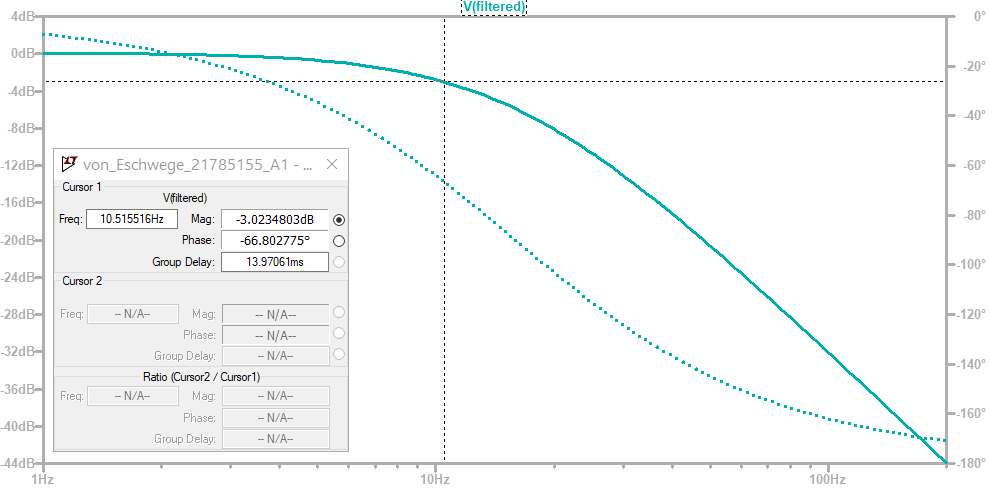
\includegraphics[width = 0.8\textwidth]{Figures/ac.png}
    \caption{Cutoff Frequency Measurement}
    \label{fig:ac}
\end{figure}

Please note:
It is a good design practice to include a unity gain op-amp to acts as a voltage buffer by clamping $V_{in-}$ against fluctuations. This design practice was considered, but ultimately rejected, as tests with and without the buffer provided outputs of equal quality. This is the case as the signal conditioning circuit already has a very high input resistance. The only notable differences resulting from the inclusion of a buffer were an increase in current drawn, as well as an increase in cost for the circuit components, as another op-amp is required. Therefore, in order to keep the current consumption below \SI{15}{mA}, as well as to use reduce cost by only using three op-amps, the voltage buffer was omitted in the final design.\\

\end{document}

